\documentclass{article}
\usepackage{tikz}

\begin{document}

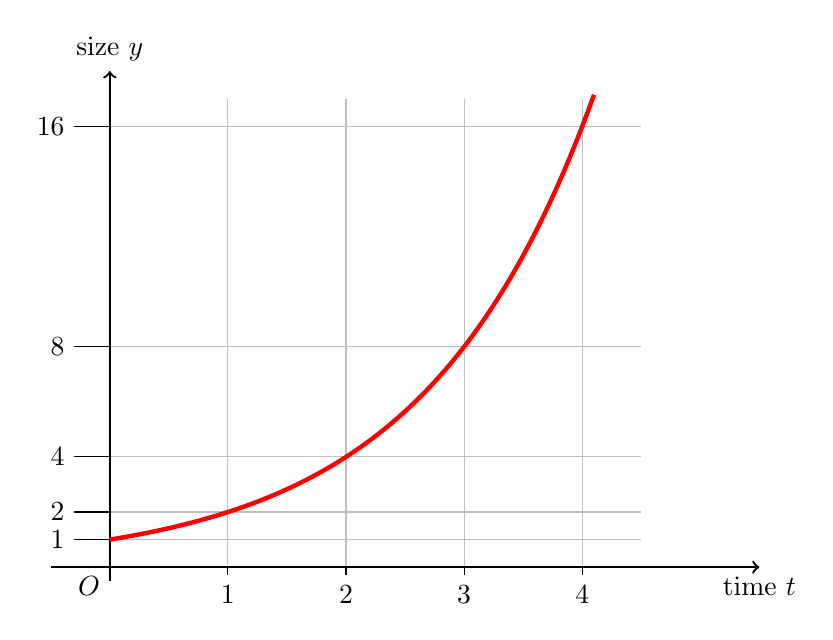
\begin{tikzpicture}[x=1.5cm,y=0.35cm]

\foreach \x in {1,...,4}{
    \draw[lightgray,thin] (\x,0)--(\x,17);
    \draw (\x,0)--(\x,-0.3) node[below] {$\x$};
}

\foreach \y in {1,2,4,8,16}{
    \draw[lightgray,thin] (0,\y)--(4.5,\y);
    \draw (0,\y)--(-0.3,\y) node[left] {$\y$};
}

\draw[->,thick] (-0.5,0)--(5.5,0) node[below] {time $t$};
\draw[->,thick] (0,-0.5)--(0,18) node[above] {size $y$};

\node[below left] at (0,0) {$O$};

\draw[red,ultra thick,domain=0:4.1,samples=100]
plot (\x,{2^\x});

\end{tikzpicture}

\end{document}
